\section{Results}
\label{sec:results}
\subsection{Main Quantitative Findings}
\begin{table*}[t]
    \centering
    \resizebox{0.95\textwidth}{!}{%
    \begin{tabular}{@{}lccc@{}}
        \toprule
        Metric Group & Metric & Value & Interpretation \\
        \midrule \midrule
        Setup & Selected directions & 20 & Instruction IDs with at least 10 single-instruction samples \\
        Setup & Multi-instruction examples & 174 & Evaluation set for representation compositionality \\
        \midrule
        Representation & Mean cosine alignment & {\bf 0.518} & Moderate directional agreement \\
        Representation & Mean R2-like score & -0.495 & Poor reconstruction quality \\
        Representation & Mean relative norm error & 0.256 & Non-trivial magnitude mismatch \\
        Representation & 95\% bootstrap CI (cosine) & [0.478, 0.543] & Stable but clearly sub-ceiling \\
        \midrule
        Pair families & Related-pair mean cosine & 0.571 & Slightly higher than unrelated \\
        Pair families & Unrelated-pair mean cosine & 0.509 & Lower average compositionality \\
        Pair families & Mann-Whitney $p$-value & 0.664 & No significant family gap \\
        \midrule
        Behavior & Joint pass rate (none / A / B / A{+}B) & 0.000 / 0.043 / 0.043 / 0.043 & Summed steering does not beat best single \\
        Behavior & Composition gain over best single & 0.000 & No additive behavioral benefit \\
        \midrule
        Transfer & TruthfulQA local additivity cosine & 0.868 & High local additivity \\
        Transfer & HellaSwag local additivity cosine & 0.919 & High local additivity \\
        \bottomrule
    \end{tabular}%
    }
    \caption{Main quantitative results. We report representation-space, behavior-space, and transfer/locality metrics. Best value for the primary representation metric is highlighted in \textbf{bold}.}
    \label{tab:main_results}
\end{table*}


\para{What is the headline result?}
As summarized in \tabref{tab:main_results}, representation-space additivity is only partially reliable. Mean cosine is 0.518 with a tight 95\% bootstrap interval [0.478, 0.543], but the mean R2-like score is negative (-0.495), which indicates poor reconstruction quality despite moderate directional agreement.

\subsection{Pairwise Compositionality Map}
\begin{figure}[t]
    \centering
    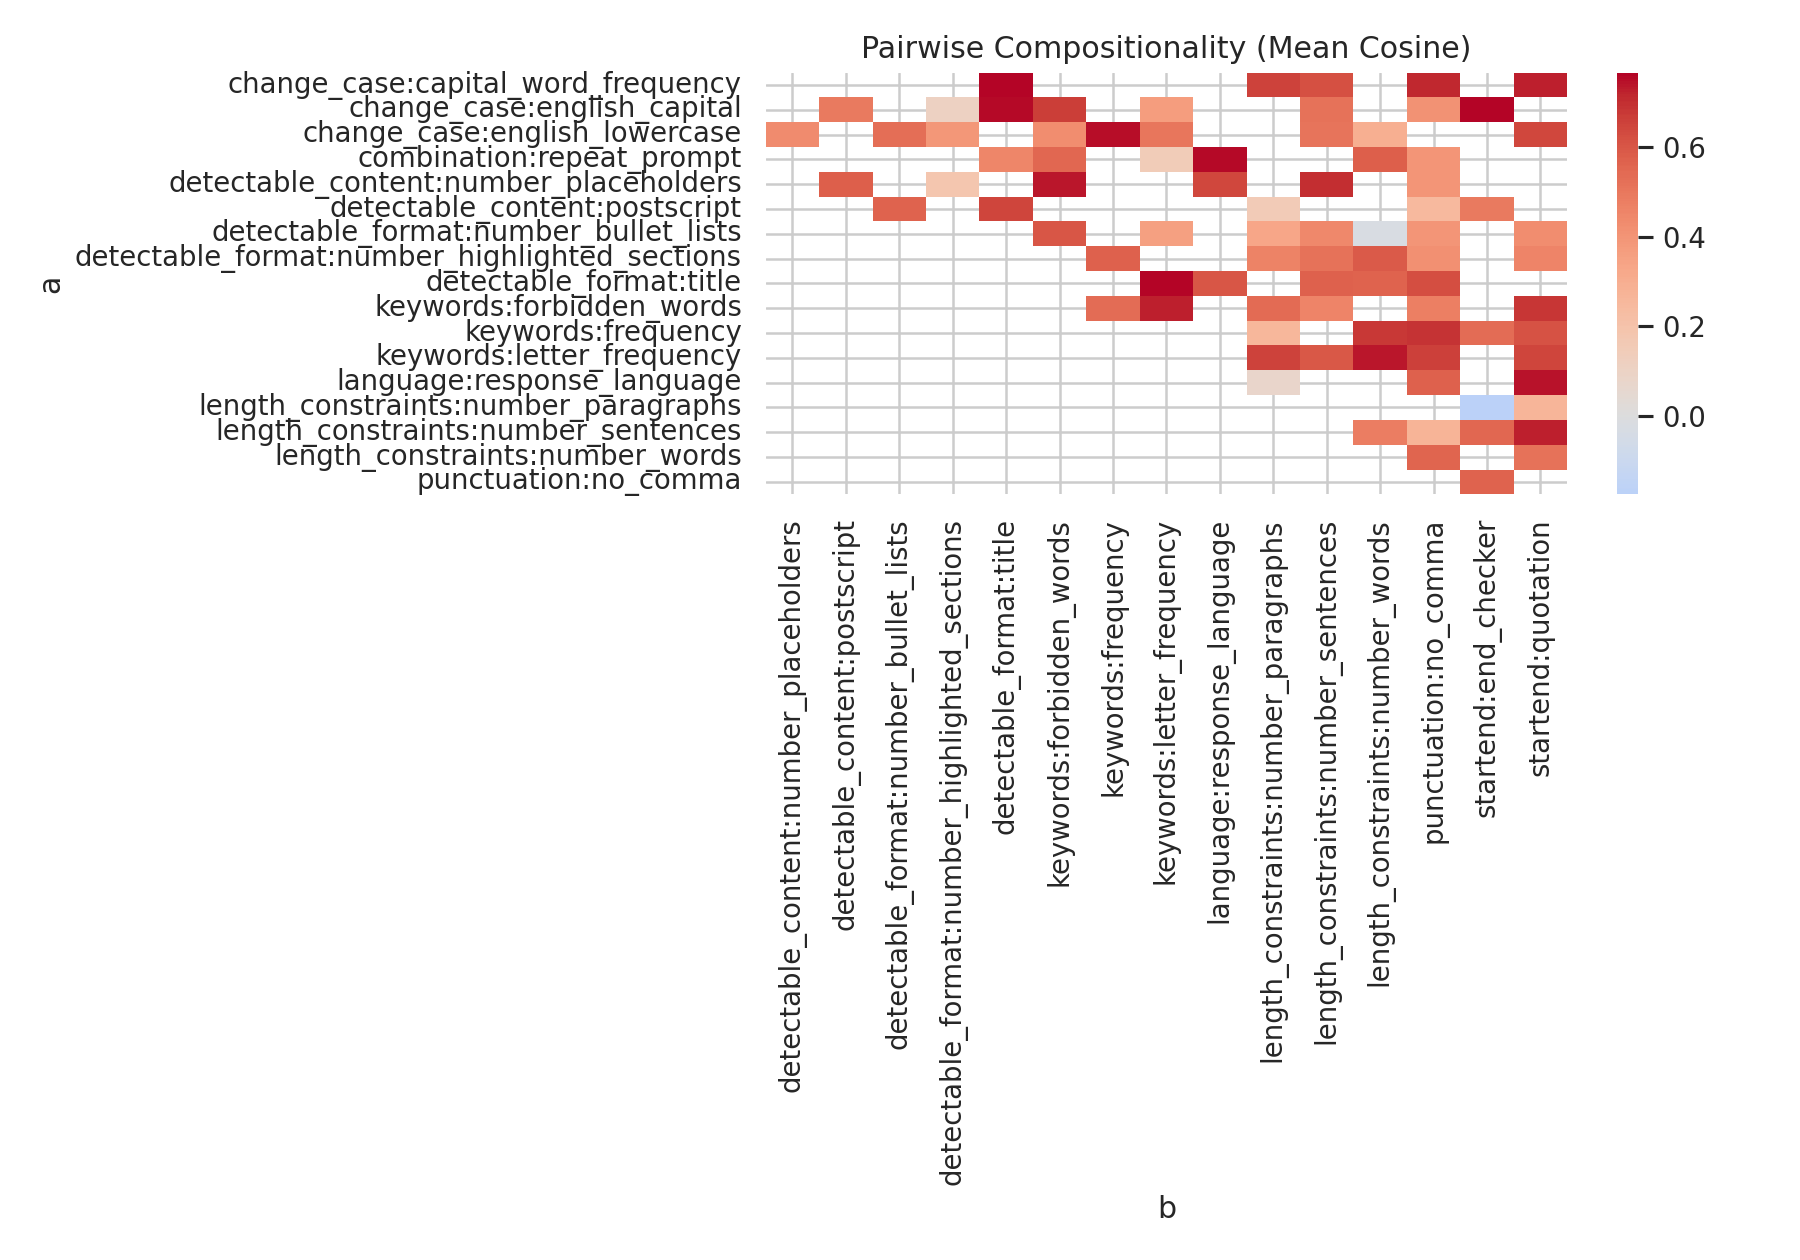
\includegraphics[width=0.95\linewidth]{figures/pairwise_compositionality_heatmap.png}
    \caption{Pairwise compositionality heatmap over instruction-direction pairs. Bright regions indicate high mean cosine alignment; dark regions indicate weak or negative composition. The map shows substantial heterogeneity rather than a uniform linear subspace.}
    \label{fig:heatmap}
\end{figure}

\begin{figure}[t]
    \centering
    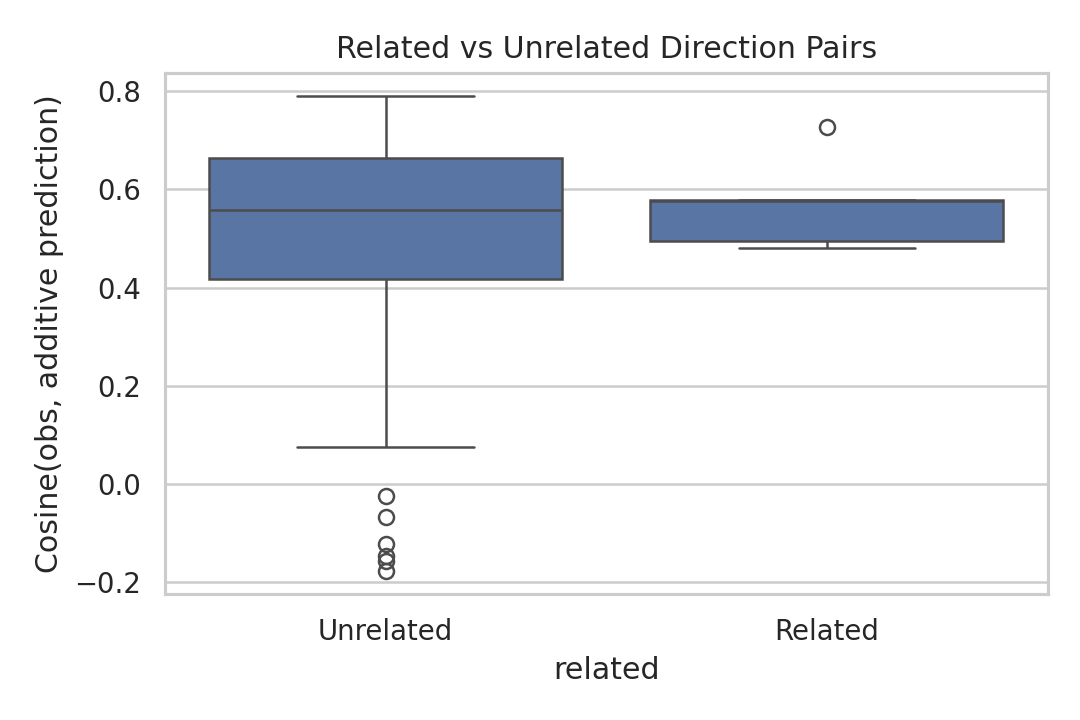
\includegraphics[width=0.80\linewidth]{figures/related_vs_unrelated_boxplot.png}
    \caption{Related vs. unrelated direction-pair cosine alignment. Related pairs have slightly higher mean (0.571 vs. 0.509), but the difference is not significant (Mann-Whitney $p=0.664$).}
    \label{fig:related_unrelated}
\end{figure}

As shown in \figref{fig:heatmap} and \figref{fig:related_unrelated}, the strongest observed pairs include \texttt{detectable\_format:title + keywords:letter\_frequency} (0.767) and \texttt{change\_case:capital\_word\_frequency + detectable\_format:title} (0.766). The weakest include \texttt{length\_constraints:number\_paragraphs + startend:end\_checker} (-0.176) and \texttt{detectable\_format:number\_bullet\_lists + length\_constraints:number\_words} (-0.025). This spread includes negative values, confirming strong pair-specific interference.

\subsection{Behavioral Compositionality}
\begin{figure}[t]
    \centering
    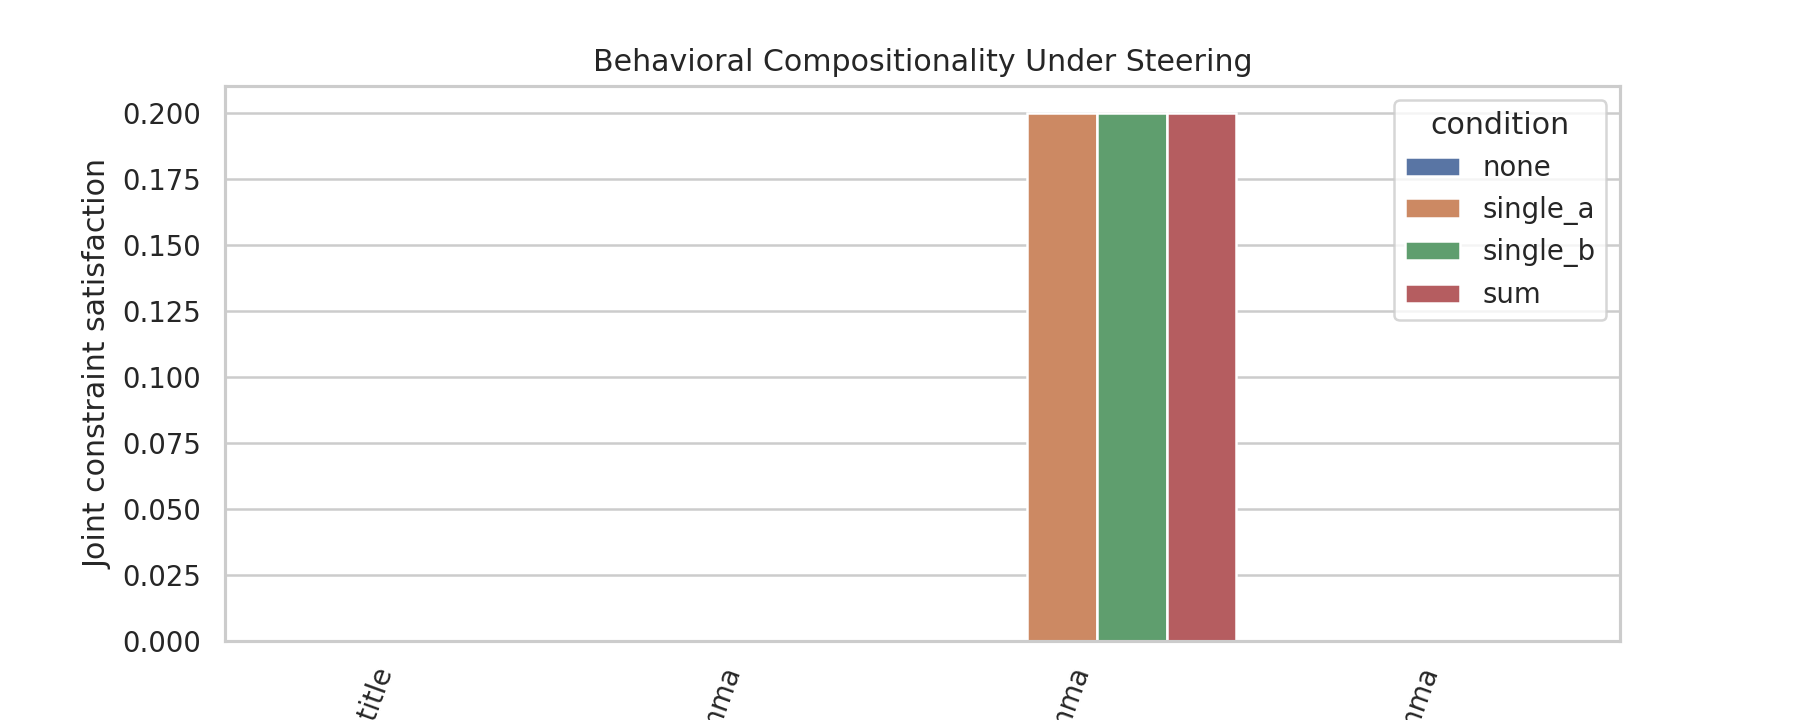
\includegraphics[width=0.80\linewidth]{figures/behavioral_compositionality.png}
    \caption{Joint two-constraint satisfaction rates under no steering, single-direction steering, and summed steering. Additive steering ($A{+}B$) matches but does not exceed the best single condition.}
    \label{fig:behavioral}
\end{figure}

Behavioral outcomes mirror representation-space fragility. Joint satisfaction is 0.000 with no steering and 0.043 for each of single-$A$, single-$B$, and $A{+}B$. The composition gain over best single is therefore 0.000, indicating no practical improvement from naive vector summation in this subset.

\subsection{Transfer and Locality}
\begin{figure}[t]
    \centering
    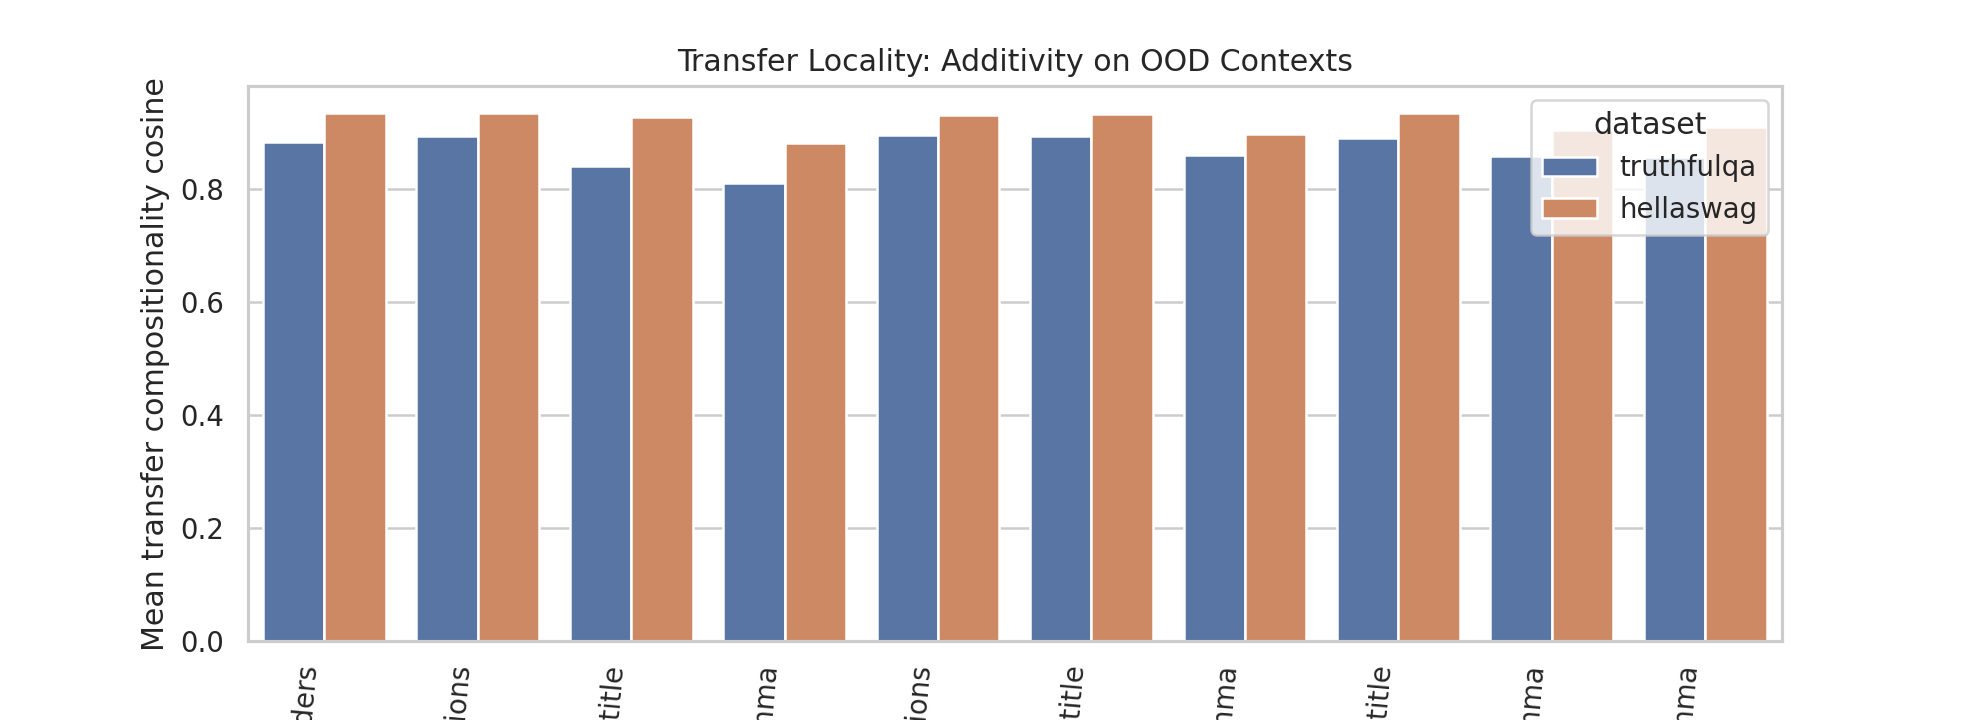
\includegraphics[width=0.80\linewidth]{figures/transfer_locality_barplot.png}
    \caption{Transfer/locality additivity on external prompts with synthetic instruction appends. Additivity is high (0.868 on TruthfulQA and 0.919 on HellaSwag), suggesting local linear structure persists even when full in-domain composition is uneven.}
    \label{fig:transfer}
\end{figure}

Transfer tests show high additivity for local perturbations (TruthfulQA 0.868; HellaSwag 0.919). Combined with weaker full-bundle results on IFEval, this pattern supports a locality interpretation: linear composition appears stronger for small contextual perturbations than for full instruction bundles.

\subsection{Reproducibility and Sensitivity}
A complete rerun with the same seed reproduces key summary metrics exactly (\texttt{summary\_run1.json} vs. \texttt{summary\_run2.json}). This deterministic match reduces concern that the observed non-compositionality is an artifact of random execution variance.
